\section{Sensitivity of the Rust Model}
\thispagestyle{plain} % surpress header on first page

As described in section \ref{generalMPEC}, the economic literature exploring the benefits of MPEC and NFXP for structural estimation is limited to studies by \cite{Su.Judd.2012}, \cite{Dube.Fox.Su.2012}, \cite{Jorgensen.2013}, \cite{Iskhakov.2016} and \cite{Dong.Hsieh.Zhang.2017}. While in these papers different economic models are considered, the set up chosen is quite clean, being mainly free of any model misspecification and allowing mostly for stable, small numerical errors in the calibration procedure. From a practical perspective and in a research setting where economic models and calibration procedures become more complex, their comparison of MPEC and NFXP is inherently limited to a world in which the modeling and calibration procedure is performed with a minimal error. In a more realistic set up that practioners commonly face where their mathematical model might be more or less off from reality and the computational model has to work with many approximations, there might actually be a larger difference between the two approaches. Those studies comparing the two approaches unanimously find that the qualitative results, i.e. the parameter estimates are the same for both and focus on the implementation side covering the speed and rate of convergence. The idea of my following simulation study is to break with the clean comparison of MPEC and NFXP by deliberately introducing some numerical error and model misspecification to test how the two approaches react to it. In this comparison I focus on qualitative aspects investigating how well the two approaches recover the true underlying model. For this a first aspect of the UQ framework comes into play. As I will also change the level of model misspecification in the Rust model a naive comparison of how the structural parameters of the underlying data generating process are recovered, as done by \cite{Su.Judd.2012}, is flawed. For this reason I rely on the previously used QoI of the counterfactual demand level at replacement cost of 11,000 Dollars. This quantity can be calculated and compared no matter the degree of model misspecification and it is an indicator on how well certain parameters in combination with some model and numerical specifications actually uncovers the predictions of the true underlying model and data generating process. A second aspect from uncertainty quantification that enters my following simulation study is the general framework of \cite{Oberkampf.2010}. They devise an approach for scientific computing in which they account for model and numerical error as well as parameter uncertainty and propagate them in various combinations through a model. This results in many different distributions of a QoI that in the end is visualized such that it is informative about the uncertainty in the QoI for those that intend to actually use the model outcome. In my simulation study I pick up key ideas of this framework and consequently investigate how changes in model specification and numerical implementation in the calibration procedure translate into the distribution of a QoI and hence its uncertainty. I do so by performing a large scale Monte Carlo simulation for the previously described Rust model. The model is well explored and can therefore be seen as the perfect benchmark for such a study whose results might probably be taken as a lower bound for the effects found of such a simulation in modern and much more complex structural models.

\subsection{The Simulation Setup}

The setup for my simulation study is inspired by that found in \cite{Iskhakov.2016}. Consequently, I stay close to the data generating process and ideas explored in section \ref{generalsetup}. First of all, I simulate 250 data sets based on the following true data generating process. The discount factor $\beta$ equals to 0.975 and the cost function $c(.)$ is linear with a scale parameter of $10^{-3}$, i.e. $c(x; \theta_{11}) = 0.001 \times \theta_{11} x$. The true cost parameters are:

\begin{equation*}
\begin{split}
& RC = 11.7257 \\
& \theta_{11} = 2.4569 . \\
\end{split}
\end{equation*}

This parametrization follows exactly the one already encountered before. The first change enters with the true transition probabilities. This change is necessary due to the nature of how the simulation of data is implemented in the ruspy package. The package gives out a data set in which the mileage state of a bus is already discretized according to a previously specified grid size. As a reminder this grid size was set to 175 in the previous setup. In this simulation I intend to investigate how a different discretization of the mileage in the same data set leads to changes in the calibration and later in the QoI. To preserve the information in the data set I have to simulate the data with a large grid size and then derive the same data set with lower grid size from it. I choose to set the grid size to 400 for the initial data generation. The previous parametrization of section \ref{generalsetup} that is optimized for a grid size of 175 will yield unproportionally small variation in mileage when used for my increased grid size. Accounting for this I adjust the true transition probabilities to be the following:

\begin{equation*}
	\resizebox{.9\hsize}{!}{$\theta_3 = \begin{pmatrix}
		0.04685 & 0.04685 & 0.22375 & 0.22375 & 0.22295	& 0.22295 & 0.00635 & 0.00635 & 0.0001 & 0.0001
		\end{pmatrix}.$}
\end{equation*}

From those 250 data sets with grid size 400 I know derive the same data sets with decreased grid size of 200 and 100. These data sets are now being calibrated with different specifications which will yield different estimated parametrizations and parameters that might cause different predictions of the QoI. Before I will explain which dimensions of the calibration procedure are tweaked, let us check on how this relates to the UQ framework from before.

As was already described the mathematical model $f(\theta)$ is the demand function in equation \ref{eq19} which in turn depends on how the Rust model is specified in order to obtain the choice probabilities $P(d|x; \theta)$ and the transition probabilities $p_3(x'|x, d; \theta_3)$ (see equation \ref{eq18}). When taking for granted that the general setup of the Rust model and its assumptions are warranted, there are several ways to easily specify the model differently which would result in changes of the two probabilities. As in the UQ framework, there might be uncertainty about the mathematical model itself which can be captured by varying functional forms of the cost function. Above that, there is uncertainty about how the parameters $\beta$ as well as $\theta$ actually look like. This is further complicated by the fact that the model does not allow us to estimate $\beta$. This leaves us quite uninformed about which $\beta$ and cost function to employ to actually explain some given data. Those circumstances already induced \cite{Rust.1987} to estimate the model several times using different specifications. In this sense my simulation will be a natural extension of his explorations. Apart from the previously explained sources of model and parameter uncertainty, there still remains variation in the model outcome stemming from the numerical implementation of the mathematical model, i.e. from the exact specification of how to solve equation \ref{eq18} with a computational model. All those sources and their effect I will account for in my simulation to a certain degree. My approach will deviate from the typical workflow in UQ, though, in some ways. Usually in uncertainty quantification (compare \cite{Smith.2013, Oberkampf.2010}) there is already some prior knowledge on how the distribution of the parameters of the model look like. This distribution is then propagated through each combination of plausible mathematical model and computational model specification. This results in a probability distribution of a QoI for each mathematical-computation-model-combination specified. In my setup, it is ad-hoc not clear how a possible distribution of the parameter vector $\theta$ might look like. Another factor is that the distribution worth propagating through the model also depends on how the mathematical and computational model are specified as the parameters are calibrated using data and a certain specification that later also affects the specification of the demand function. A further factor that is not linked directly to the demand function but potentially affects the calibration procedure and hence the plausible distribution of $\theta$ is the choice of MPEC or NFXP. This remains to be shown, though. Resting on the previous discussion, my approach can be summarized like the following. I combine possible errors in the mathematical and computational representation in the Rust model. These errors directly affect the demand function by itself and further do so indirectly by different calibration results that yield plausible, varying distributions of $\theta$ that affect the QoI. I further add another source of parameter uncertainty that stems from the calibration procedure itself and hence only changes the QoI through the variation in parameters. I test two possible numerical errors which are the difference in using either MPEC or NFXP as well as relying on numerical first order derivatives for the likelihood function as opposed to analytical ones. By this I perform an uncertainty quantification of the Rust model in which I incorporate different sources of error and in which the only information on the parametrization of the model comes from the model itself through its calibration. The goal of the approach is twofold. It shall uncover whether NFXP and MPEC might yield different qualitative results when facing unfavourable conditions while at the same time perform a broader check of the model implications when facing reasonable discrepancies in the mathematical and numerical model specification. Hence, it is supposed to be a comprehensive approach that gives as much valuable information to policy makers as possible. \paragraph{}

I will now explain the exact steps taken to arrive at the results presented below. I run a Monte Carlos simulation with 250 runs each per specification. As a benchmark case I estimate the parameters when relying on the true specification of the model. This means that I run the estimation on the 250 data sets with gird size 400, linear cost function, a $\beta$ of 0.975 as well as analytical first order derivatives of the likelihood function. This first specification I call the "correctly specified" in the following. This and all the other specifications are hence estimated on 250 data sets and this once per approach MPEC and NFXP. This simulation is equivalent to a parametric bootstrap, as noted by \cite{Su.Judd.2012}, which allows me to obtain sample statistics for the parameters. While the 250 runs do not allow me to obtain exactly unbiased estimates of true parameters, I still do not opt for more runs as the sheer amount of different specifications I consider would make it too computationally expensive given the limited time during my thesis. Further it makes it more comparable to the set up in \cite{Iskhakov.2016} and \cite{Su.Judd.2012} as they also solely simulated 250 data sets per specification. Due to estimating the model twice (once with MPEC and once with NFXP) per specification 500 runs are performed. So which specifications do I use? The specifications differ in the degree of model misspecification (or flexibility) and numerical error. The model uncertainty is introduced by allowing more flexibility in the cost function than the true data generating process actually displays. The true cost function is linear but I also allow the optimizers to employ more flexible cost function. Specifically, quadratic cost $c(x; \theta_{11}, \theta_{12}) = \theta_{11}x + \theta_{12}x^2$ or cubic cost $c(x; \theta_{11}, \theta_{12}, \theta_{13}) = \theta_{11}x + \theta_{12}x^2 + \theta_{13}x^3$ are possible. Additionally, I add the dimension of a wrongly specified $\beta$. In my setup it is therefore possible that the estimation is based on $\beta = 0.985$ although it truly is equal to 0.975.

A numerical error is introduced in two ways. While the true data generating process conveys all its information on the mileage state into a grid of 400 points, I deliberately estimate the model parameters with some loss of this information. As already mentioned, this is accounted for by running the calibration after discretizing the mileage state further from 400 to either 200 or 100 grid points. Lastly, I give the option of the realistic feature that the economic model and the estimation procedure give rise to a likelihood function that has to rely on numerical first order derivatives as opposed to analytical ones. This is the only part of the specifications that affects the QoI solely through the calibration of the structural parameters.

Clearly, it might be possible that several of those misspecifications occur at the same time and that the uncertainty introduced in the QoI might depend on this. For that reason, I build the Cartesian product of all those single misspecifications to estimate each of its possible combinations which leaves me with 36 specifications for which I separately estimate the parameters for 250 data sets using the NFXP and MPEC, respectively. A list of all specifications can be found in Table \ref{table4} in the appendix B. All this amounts to 18,000 runs for which the model is calibrated and the resulting parameters are taken to calculate the expected implied demand for bus engines for the counterfactual level of replacement cost at 11,000 Dollars. Selected results of this procedure are presented in the following section.

\subsection{The Results}

In the first step, we look at some partial sensitivity explorations to get a sense of how the QoI reacts to small changes in the model setup. This means that at first I only look at those specifications in which I deviate from the correctly specified model in only one dimension. This is I am either tweaking the model dimension, i.e. just the cost function and/ or $\beta$ or I change the numerical dimension consisting of the grid size and the use of numerical gradients. Before I do so let us fill up on the missing ingredient of the setup discussion from before. The setup for MPEC is exactly chosen as it was described in section \ref{generalsetup}. Again I use IPOPT as a solver with the tolerances specified as before. My initial intention to keep the setup as close to the one in \cite{Iskhakov.2016} as possible had to be eased a bit for the NFXP, though. This is due to malperformance of the initial setup that I employ to replicate the results in \cite{Iskhakov.2016} when facing more flexible cost functions. This is the starting point of the following section.

\subsubsection{The Partial Perspective}

\begin{figure}[!b]
	\caption{Distribution of the QoI}
	\vspace*{-4mm}
	\centering
	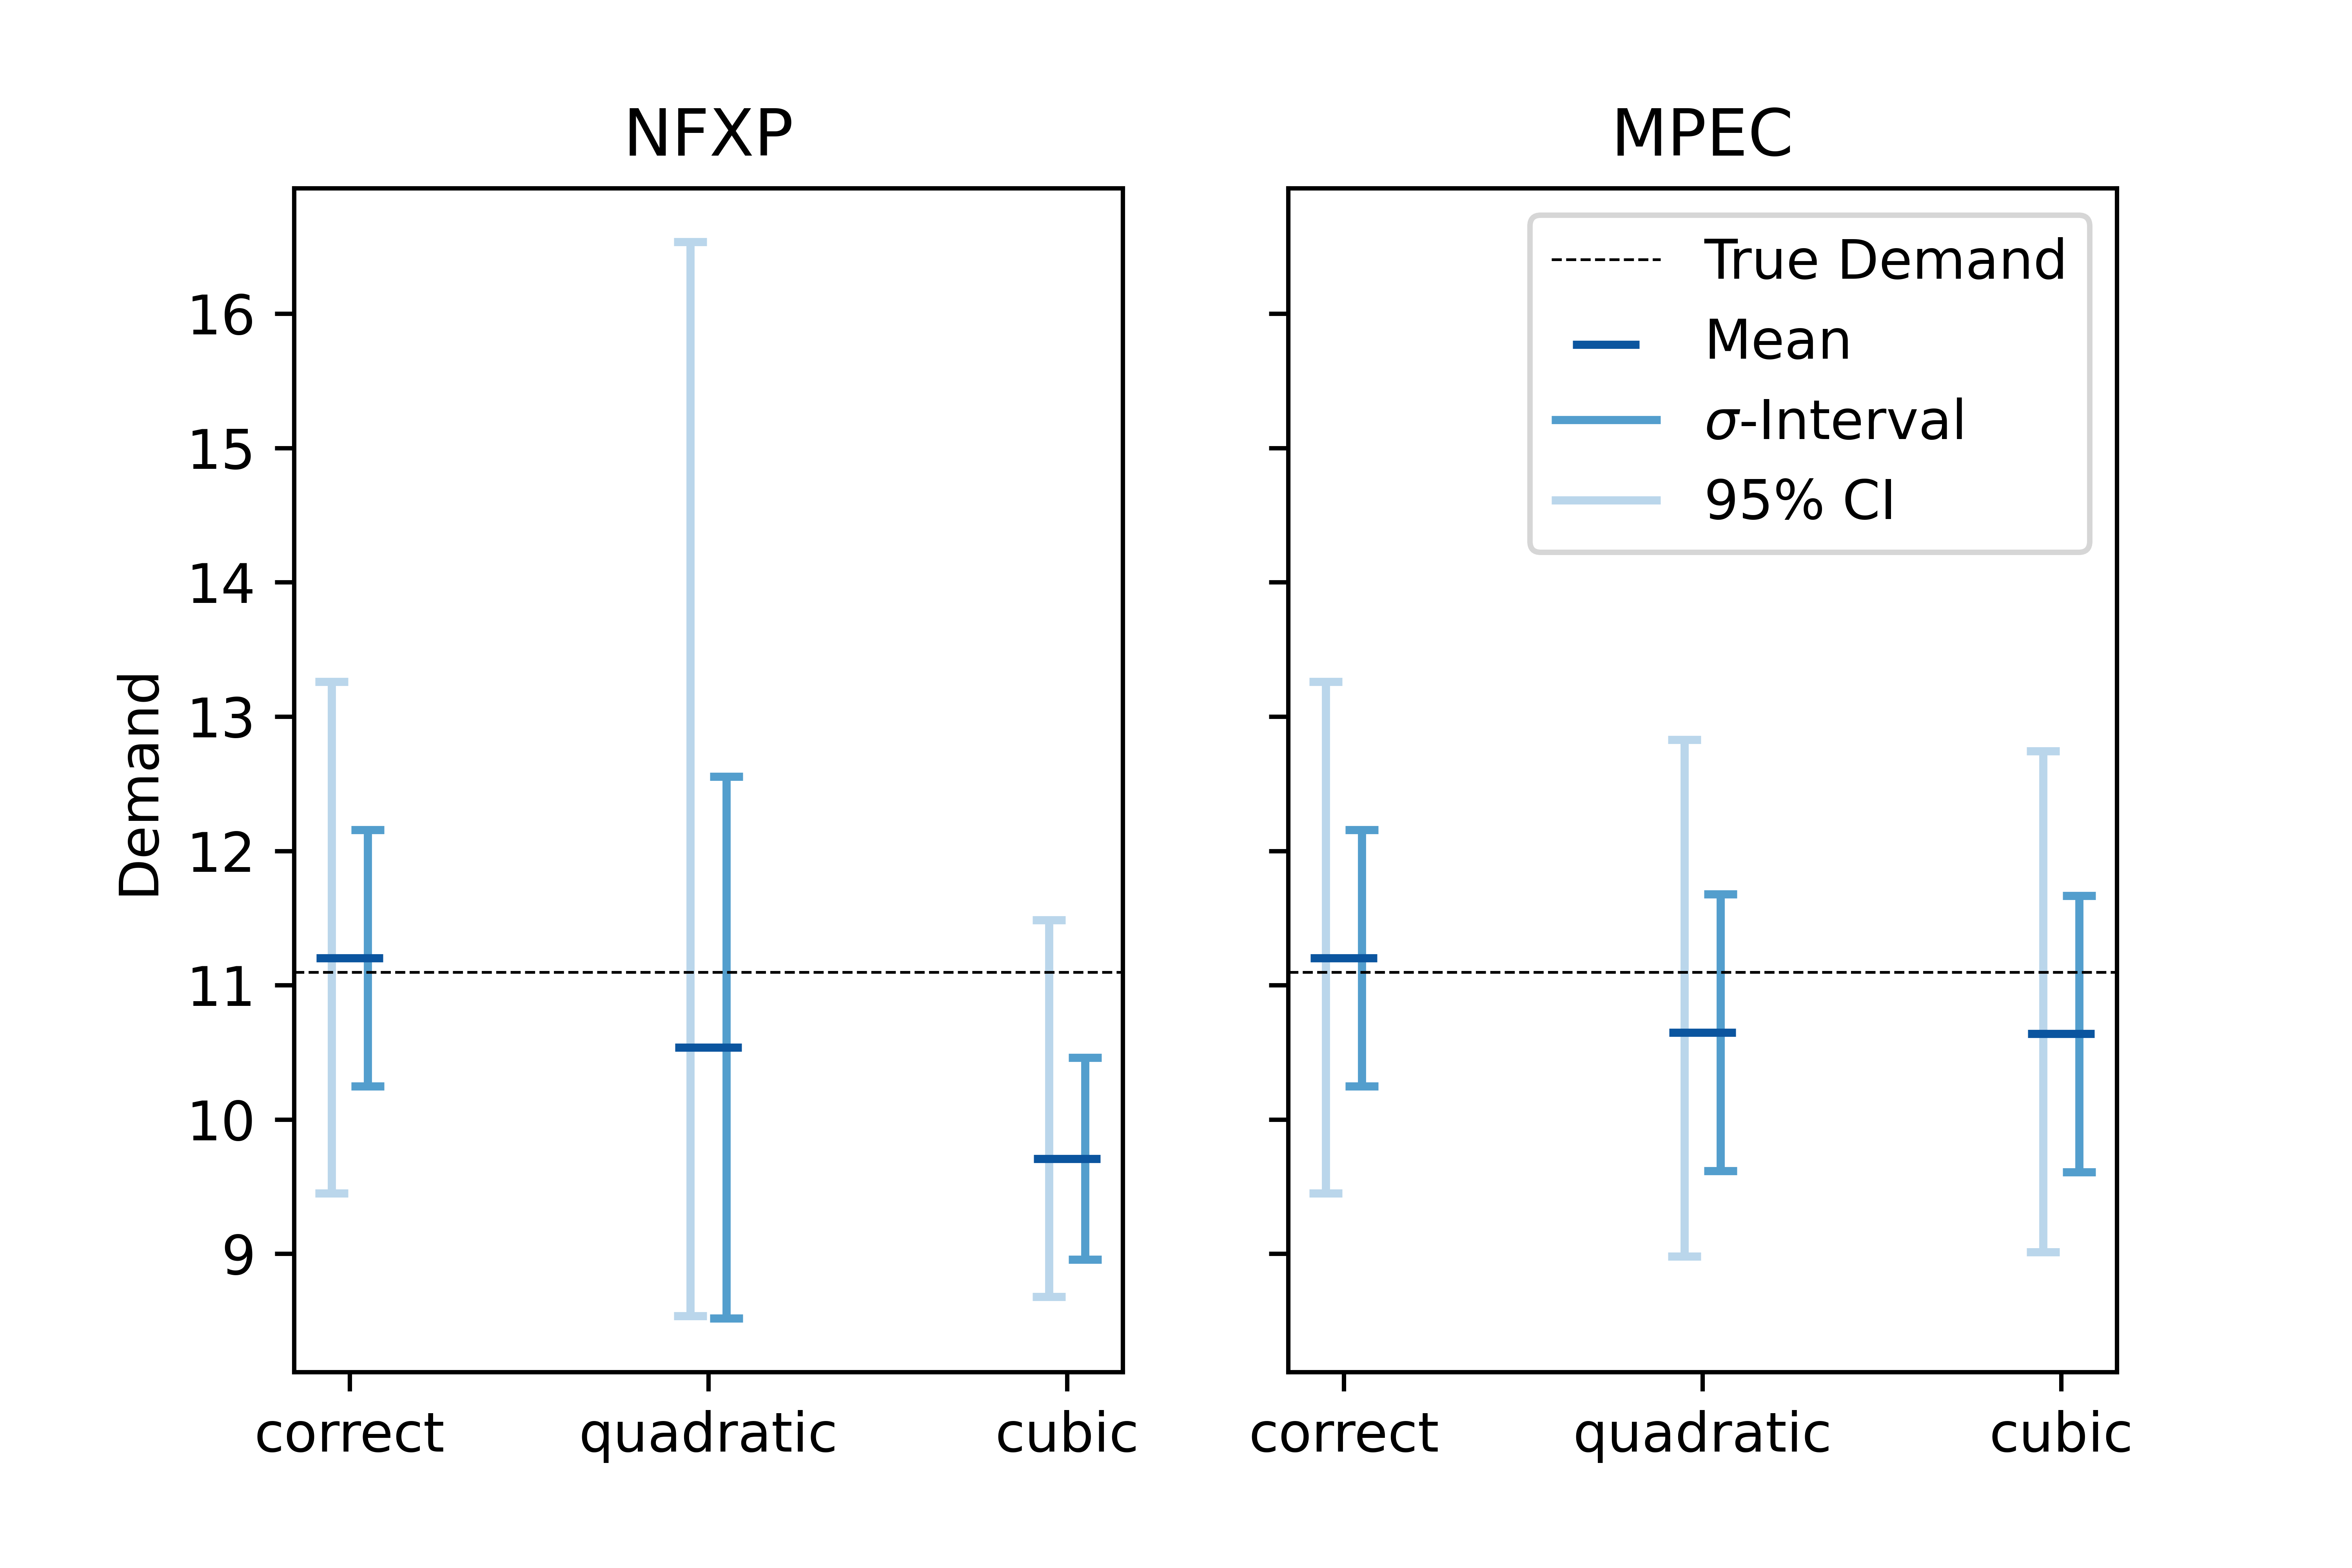
\includegraphics[scale=0.9]{../figures/figure_5.png}
	\label{figure5}
\end{figure}

The first results are those coming from the specifications in which I only add more flexibility to the cost functions that are then used to calibrate the Rust model. Apart from that the model stays correctly specified. In Figure \ref{figure5}, I present some summary statistics for the QoI depending on which specification is used and for NFXP and MPEC separately. This same kind of figure with its labeling will follow us along for several explorations which is why the legend in the subsequent figures will be dropped. Figure \ref{figure5} shows the correctly specified model at the very left as a benchmark case for both NFXP and MPEC. For this and the other specifications the mean of the QoI across the 250 runs, as well as its 95\% confidence and standard deviation interval are reported \footnote{For the bootstrap confidence interval the percentile bootstrap is used (compare \cite{Davison.1997} chapter 5).}. As already noted before the mean of the QoI for the correctly specified model does not exactly match the true value of the QoI. This is the case as there are not sufficiently many Monte Carlo runs such that the mean of the structural parameters are estimated with some small sample bias which translates into the QoI. As a reminder the true QoI is derived from the true underlying model and its true structural parameters. In our setting the true QoI is the following:

\begin{equation*}
	QoI_{true} = 11.095.
\end{equation*}

\begin{figure}[!b]
	\caption{Distribution of the QoI}
	\vspace*{-4mm}
	\centering
	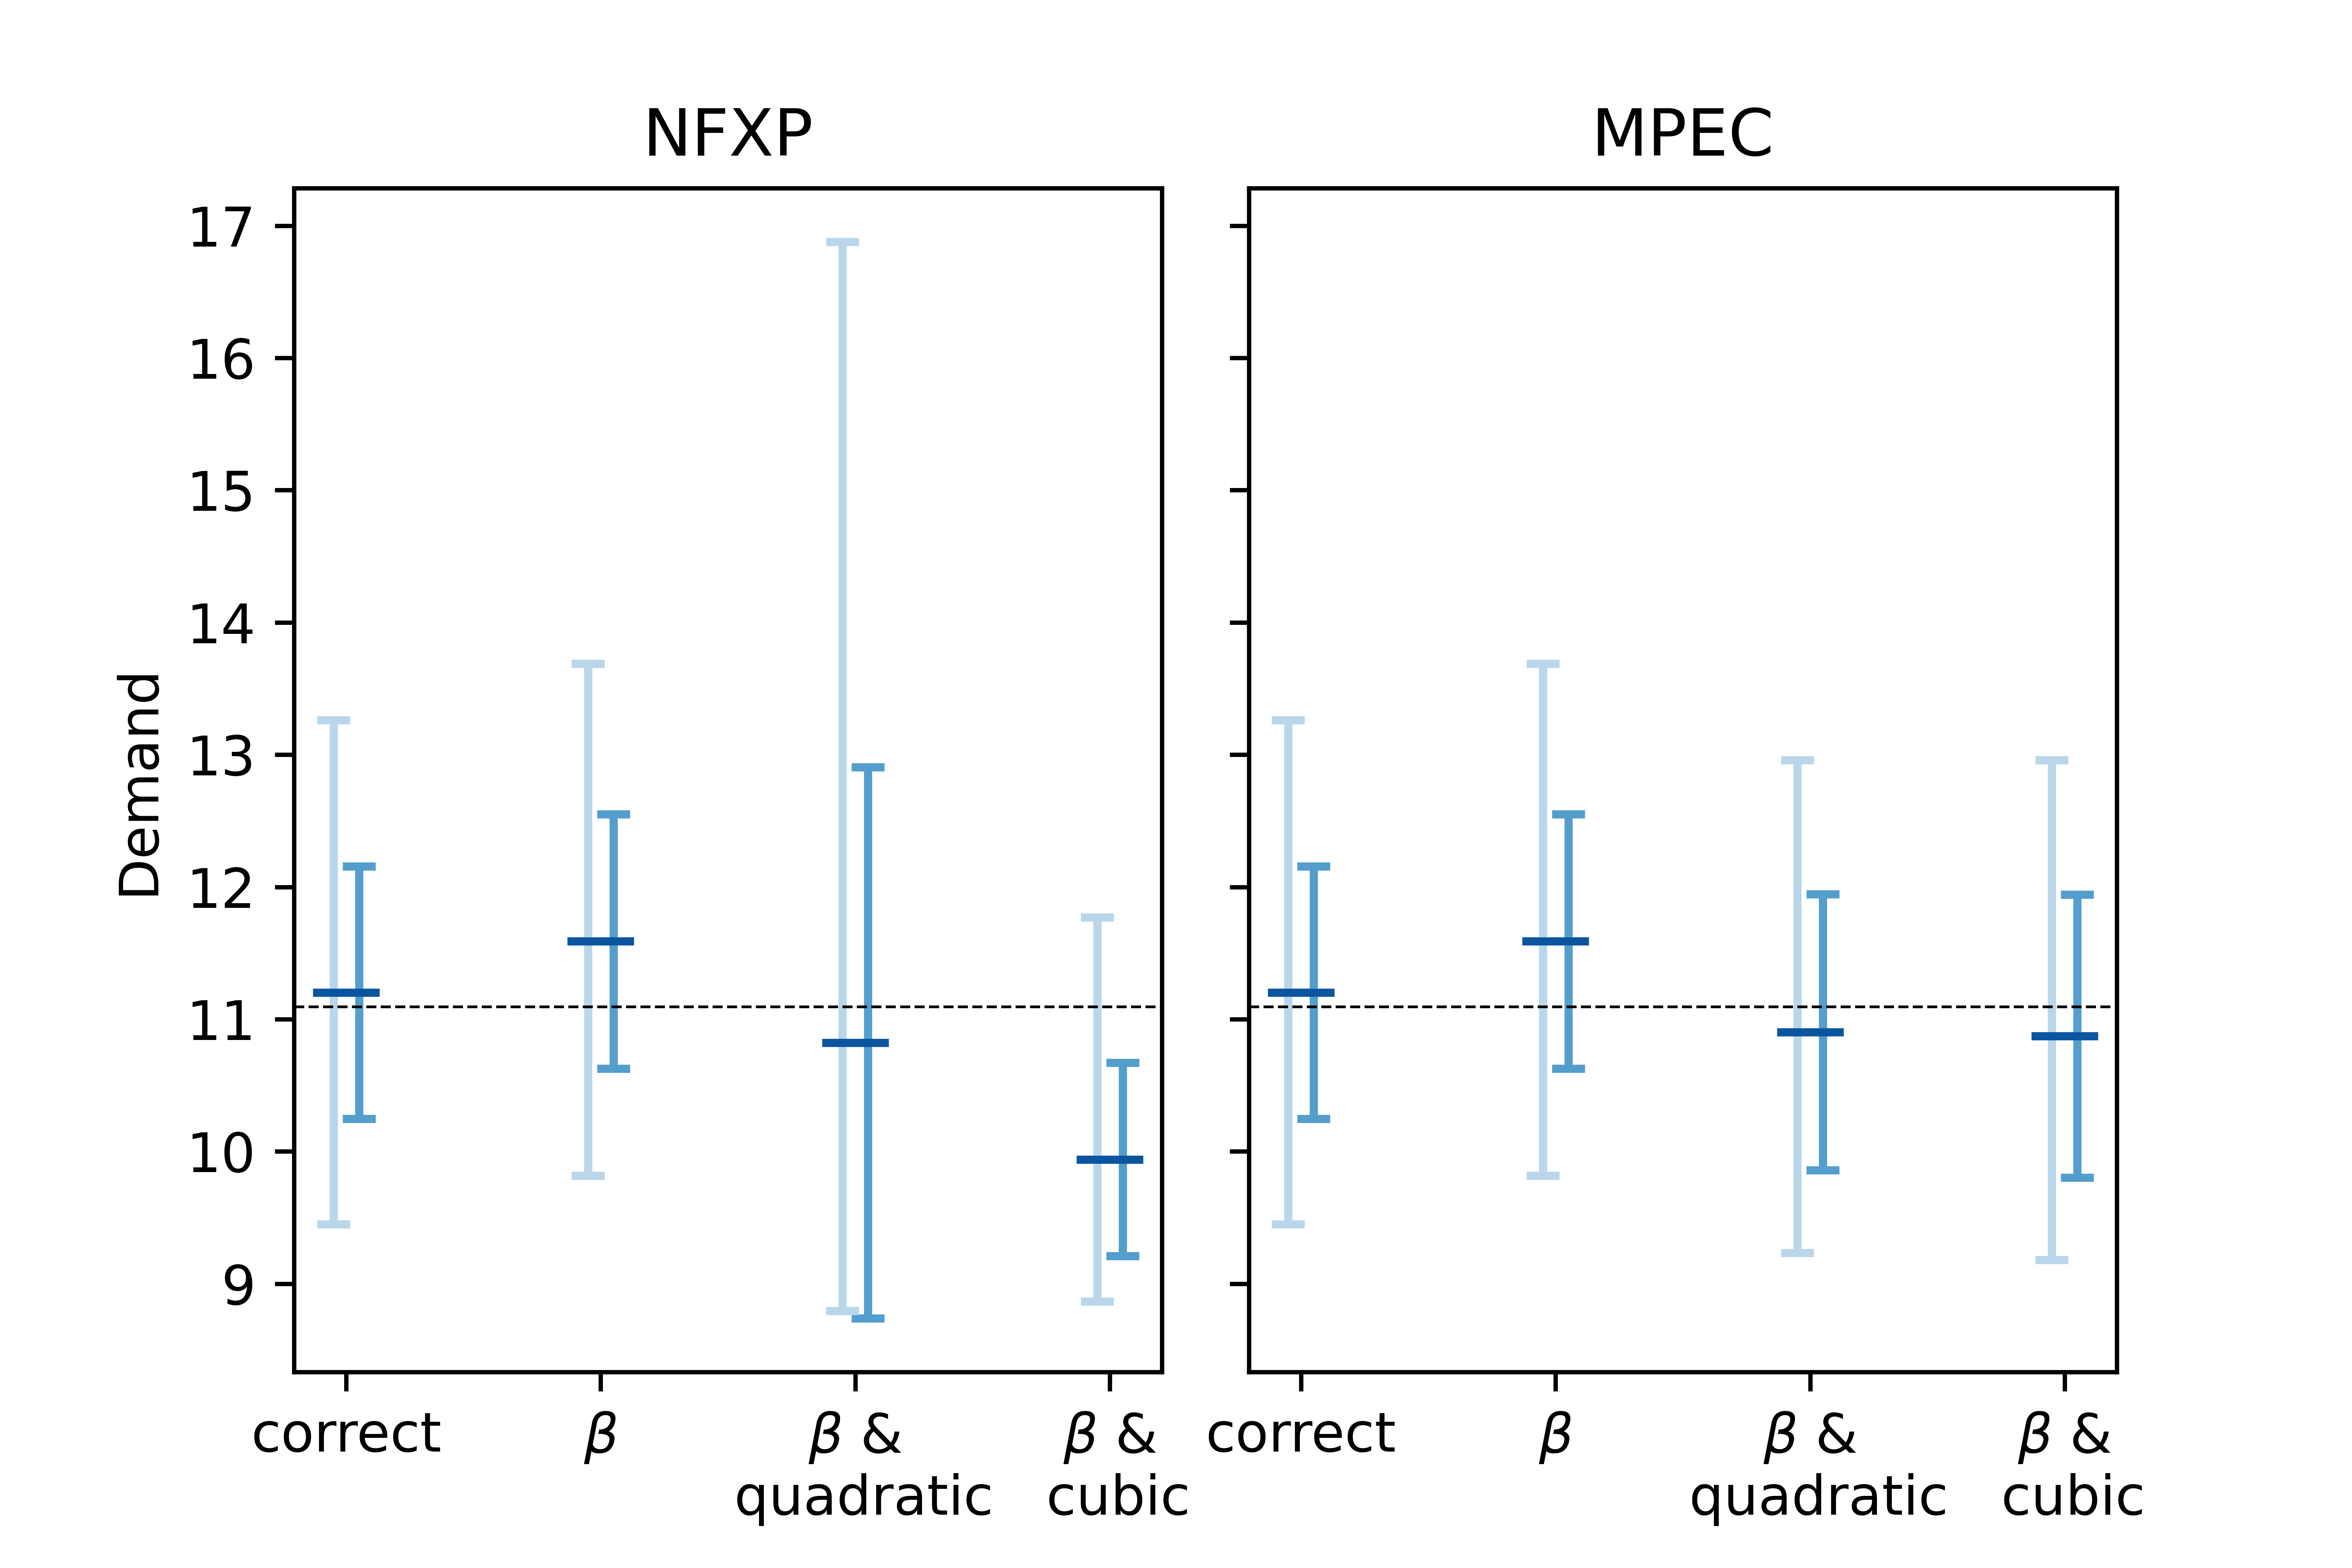
\includegraphics[scale=0.9]{../figures/figure_6.png}
	\label{figure6}
\end{figure}

When using the correctly specified model, as expected, NFXP and MPEC yield virtually the same results for all three key statistics. The mean comes in at $11.203$ while the one standard deviation interval spreads from $10.248$ to $12.157$ with the confidence interval being equal to $(9.449, 13.261)$. We move to the specification in which the correct model is maintained with the exception that the calibration procedure now assumes the cost function to be more flexible by adding a possible quadratic term. This reveals an interesting difference between the NFXP and MPEC which I tried to eliminate but could not entirely. Firstly, the means for the QoI for both approaches now underestimate the true one while the NFXP does so more strongly than MPEC. NFXP yields $10.537$ while MPEC estimates $10.646$. This difference stems from different estimates for all three structural cost parameters. Both approaches have a convergence rate of 100 percent but when comparing the estimates per run one can observe that the two approaches systematically find different solutions in every run. The NFXP implementation that yields these results is actually obtained by using the scipy implementation of the L-BFGS-B (\cite{scipy.2020}) with its default tolerances. Apart from that the setup of the NFXP algorithm used here is the same as in section \ref{generalsetup}. Solely I replace the BHHH by the above mentioned solver \footnote{In an initial try I ran the whole simulation with the BHHH with the tolerances exactly set to the ones from section \ref{generalsetup}. This produced the results in Figure \ref{figure12} which are very far off. After fruitless experimenting with the tolerances of the optimizer and the fixed point algorithm, I switched to the L-BFGS-B. When using that one as well, the results do not change a lot when varying the tolerances which is why in the ende I simply adapt the default settings for the optimizer and the tolerances from section \ref{generalsetup} for the fixed point calculation.}. The figure further reveals that the variation in estimates for the QoI is a lot larger when relying on the NFXP as opposed to MPEC. This pattern seems to flip around, though, when assuming the cost function to have a cubic form. The underestimation of the QoI in the case of NFXP becomes even more pronounced, while all key statistics stay roughly constant when applying MPEC.

This qualitative difference between the two approaches is surprising as the theoretically both solve the same problem and find the same results as proven by \cite{Su.Judd.2012}. In practice, though, the calibration procedure in the Rust model cannot be solved analytically and hence different problem formulations can react differently on numerical solving. A further complicating factor is posed by the use of different optimizers for the two approaches. Internally, their functioning clearly differs as for instance both rely in my case on a numerical approximation of the Hessian matrix which already differs analytically due to the competing problem formulations but will even differ more due to contrasting approximation techniques. It is entirely possible that despite my experimentation with tolerances, the NFXP can be set up such that it obtains the same results as MPEC in my specifications. At the same time, though, as the two approaches are promoted as a competitors as opposed to complements, many practioners might rely on only either of the two approaches which will possibly leave them with the single results of MPEC or NFXP as I found them. Clearly, looking separately at them, they both do not appear implausible. Yet, having estimated the other approach as well would convey additional information about the quality of the other.

From an uncertainty perspective it is interesting to note that giving more flexibility in the cost function to the estimation procedure it does not simply estimate linear cost but exploits the two additional terms in the cost function. This results in a downward bias for the QoI irrespective of using the NFXP or MPEC. Looking at MPEC alone, it seemingly shifts the distribution of the QoI.






\begin{figure}[H]
	\caption{Distribution of the QoI}
	\vspace*{-4mm}
	\centering
	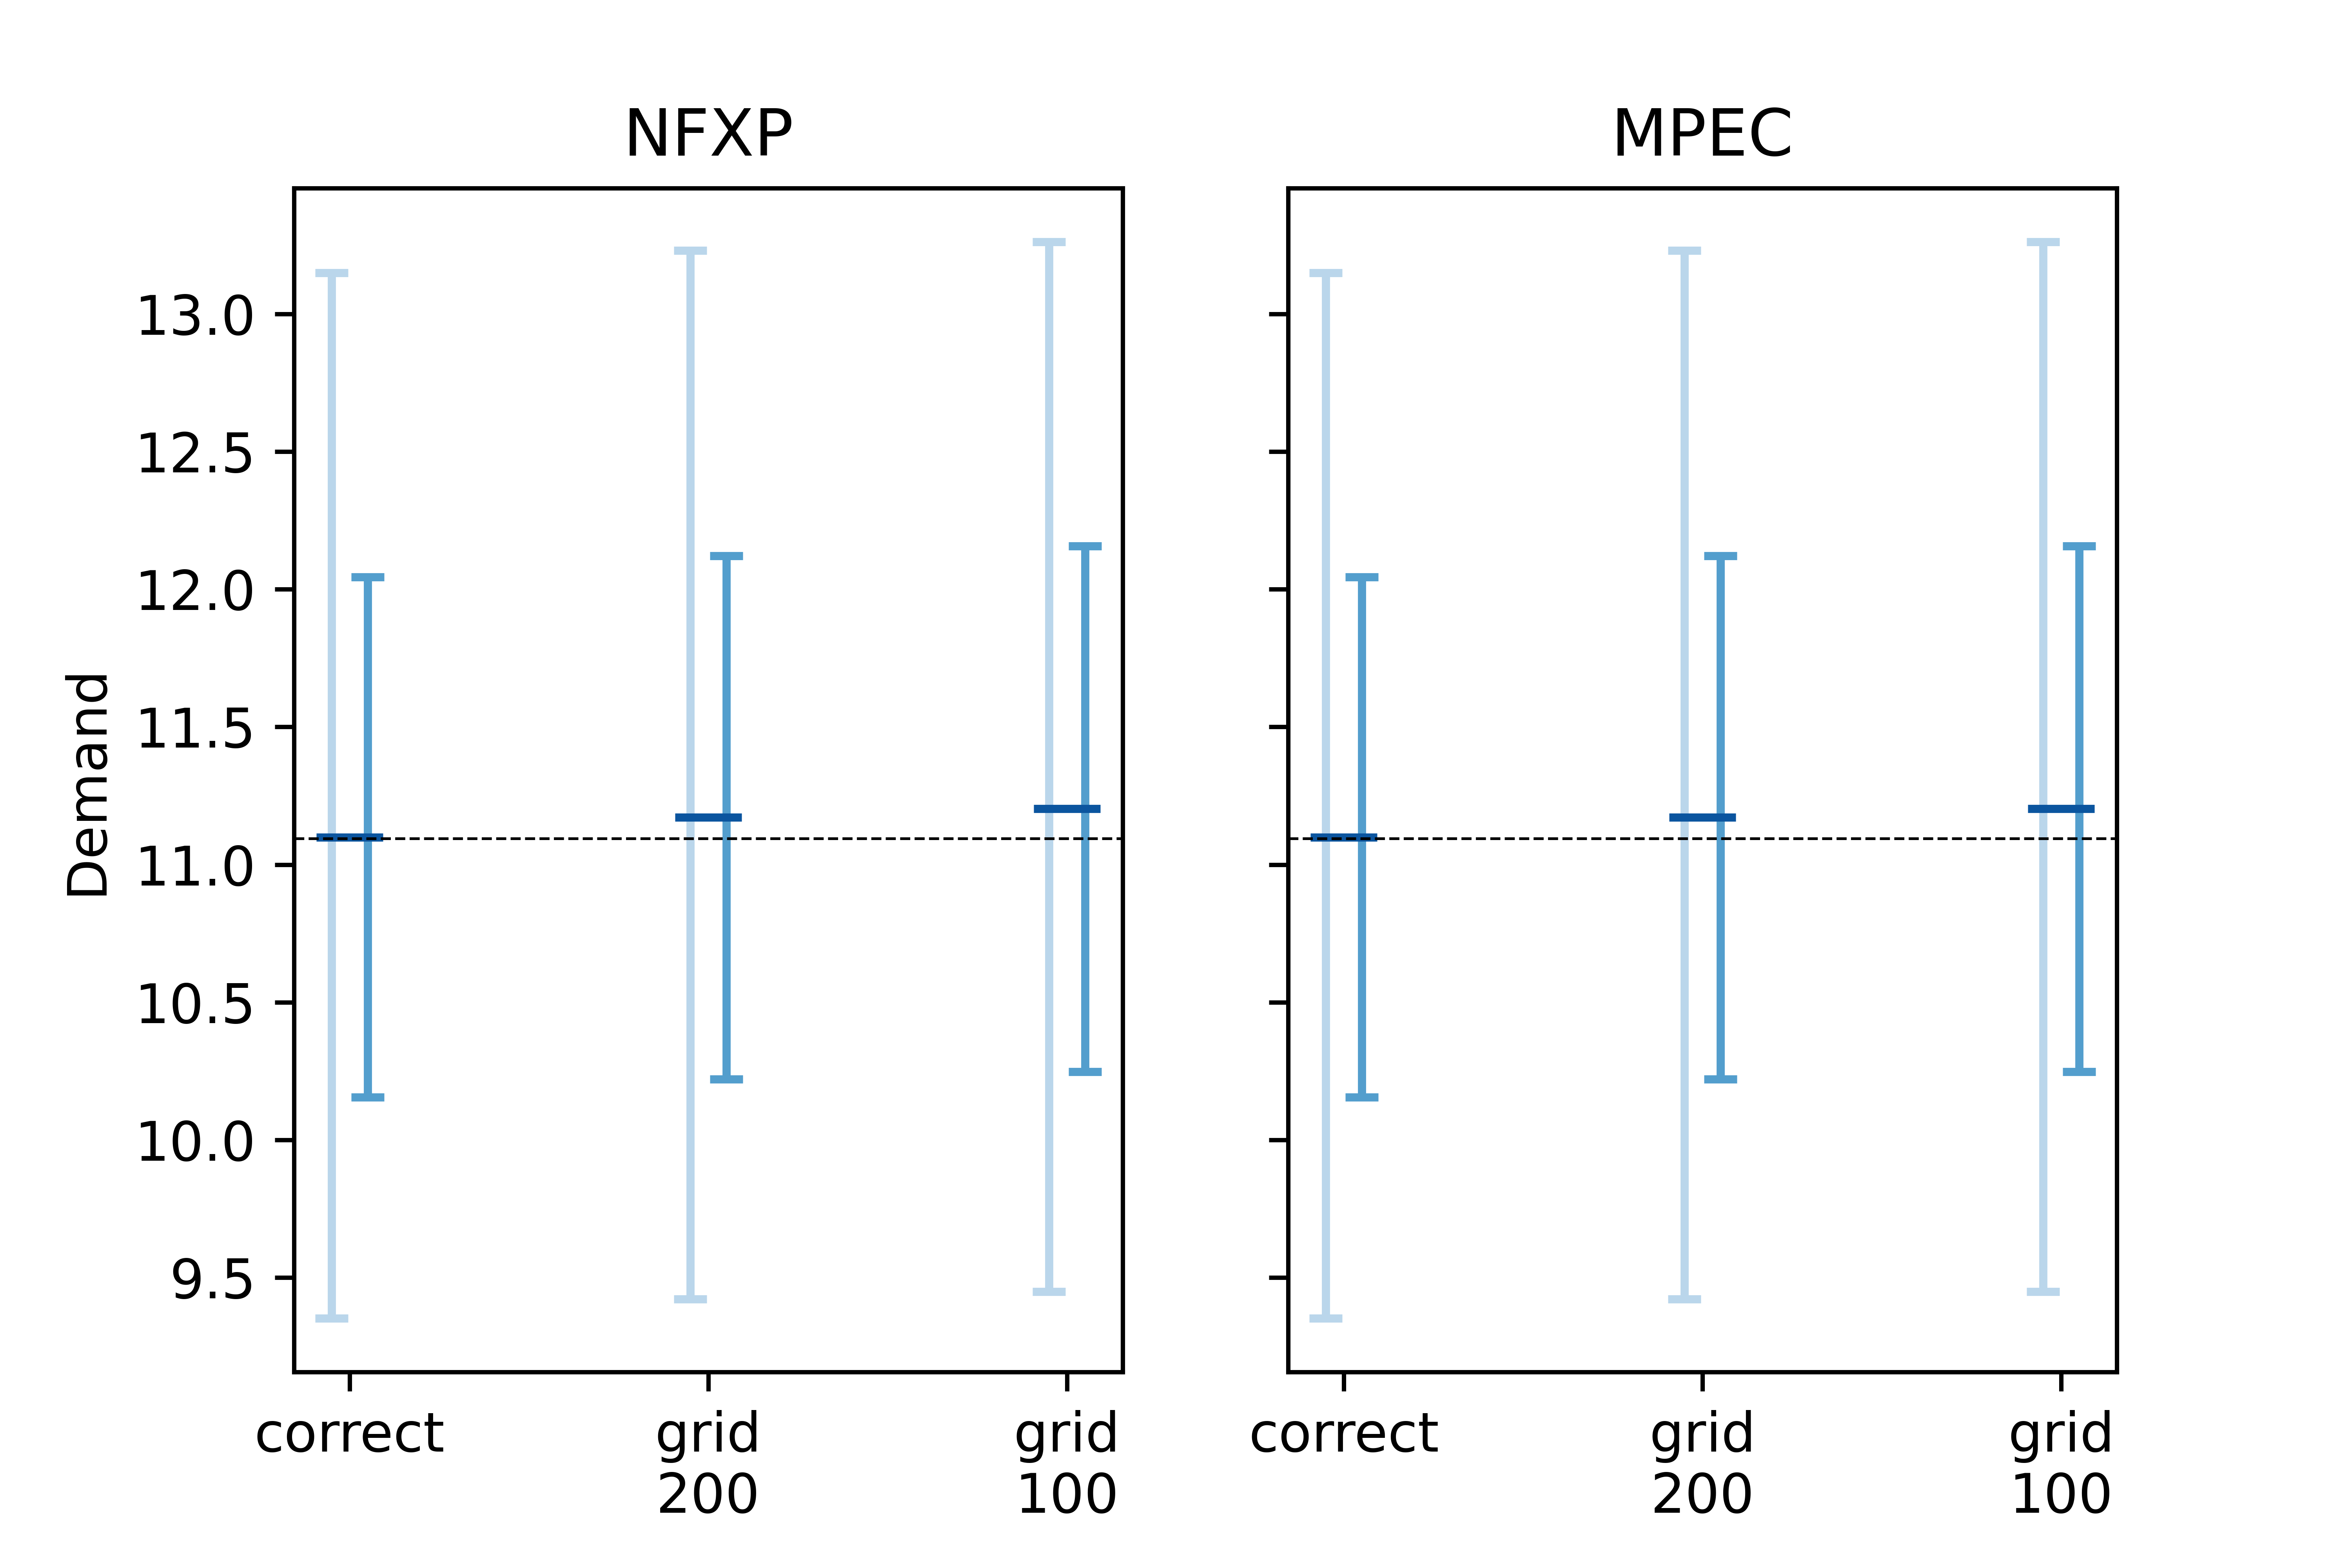
\includegraphics[scale=0.9]{../figures/figure_7.png}
	\label{figure7}
\end{figure}

\begin{figure}[H]
	\caption{Distribution of the QoI}
	\vspace*{-4mm}
	\centering
	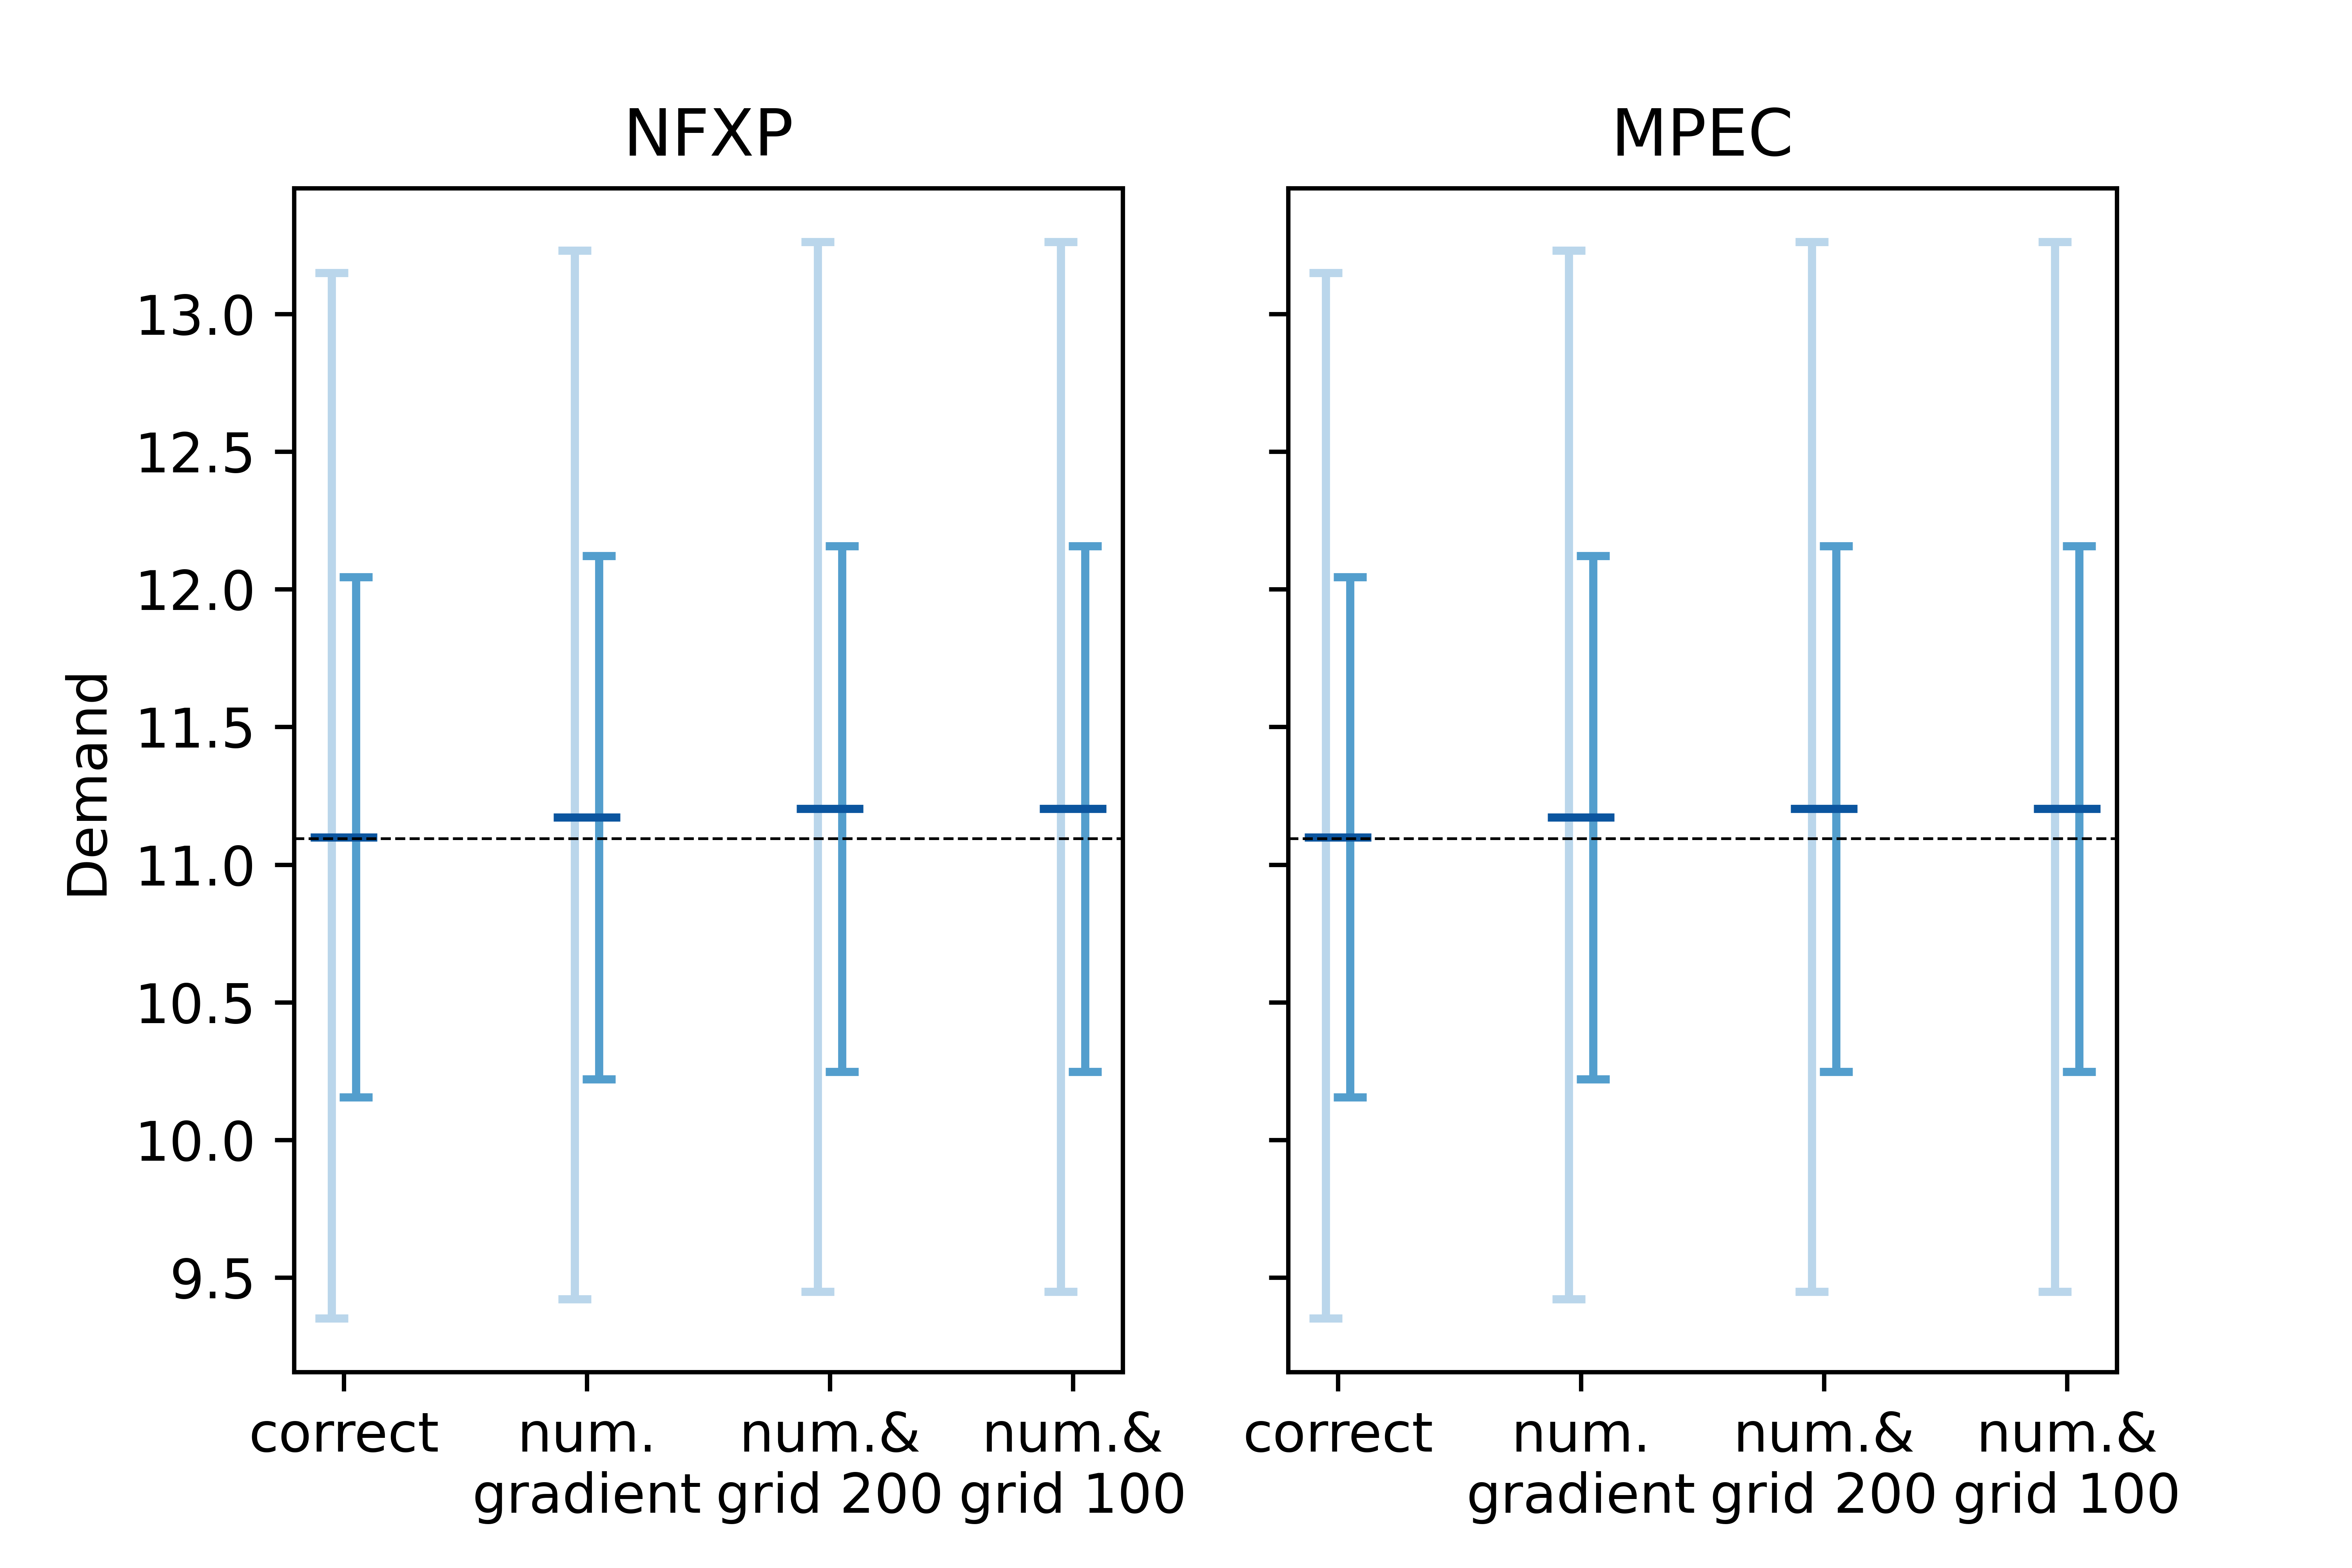
\includegraphics[scale=0.9]{../figures/figure_8.png}
	\label{figure8}
\end{figure}

\begin{figure}[H]
	\caption{Distribution of the QoI}
	\vspace*{-4mm}
	\centering
	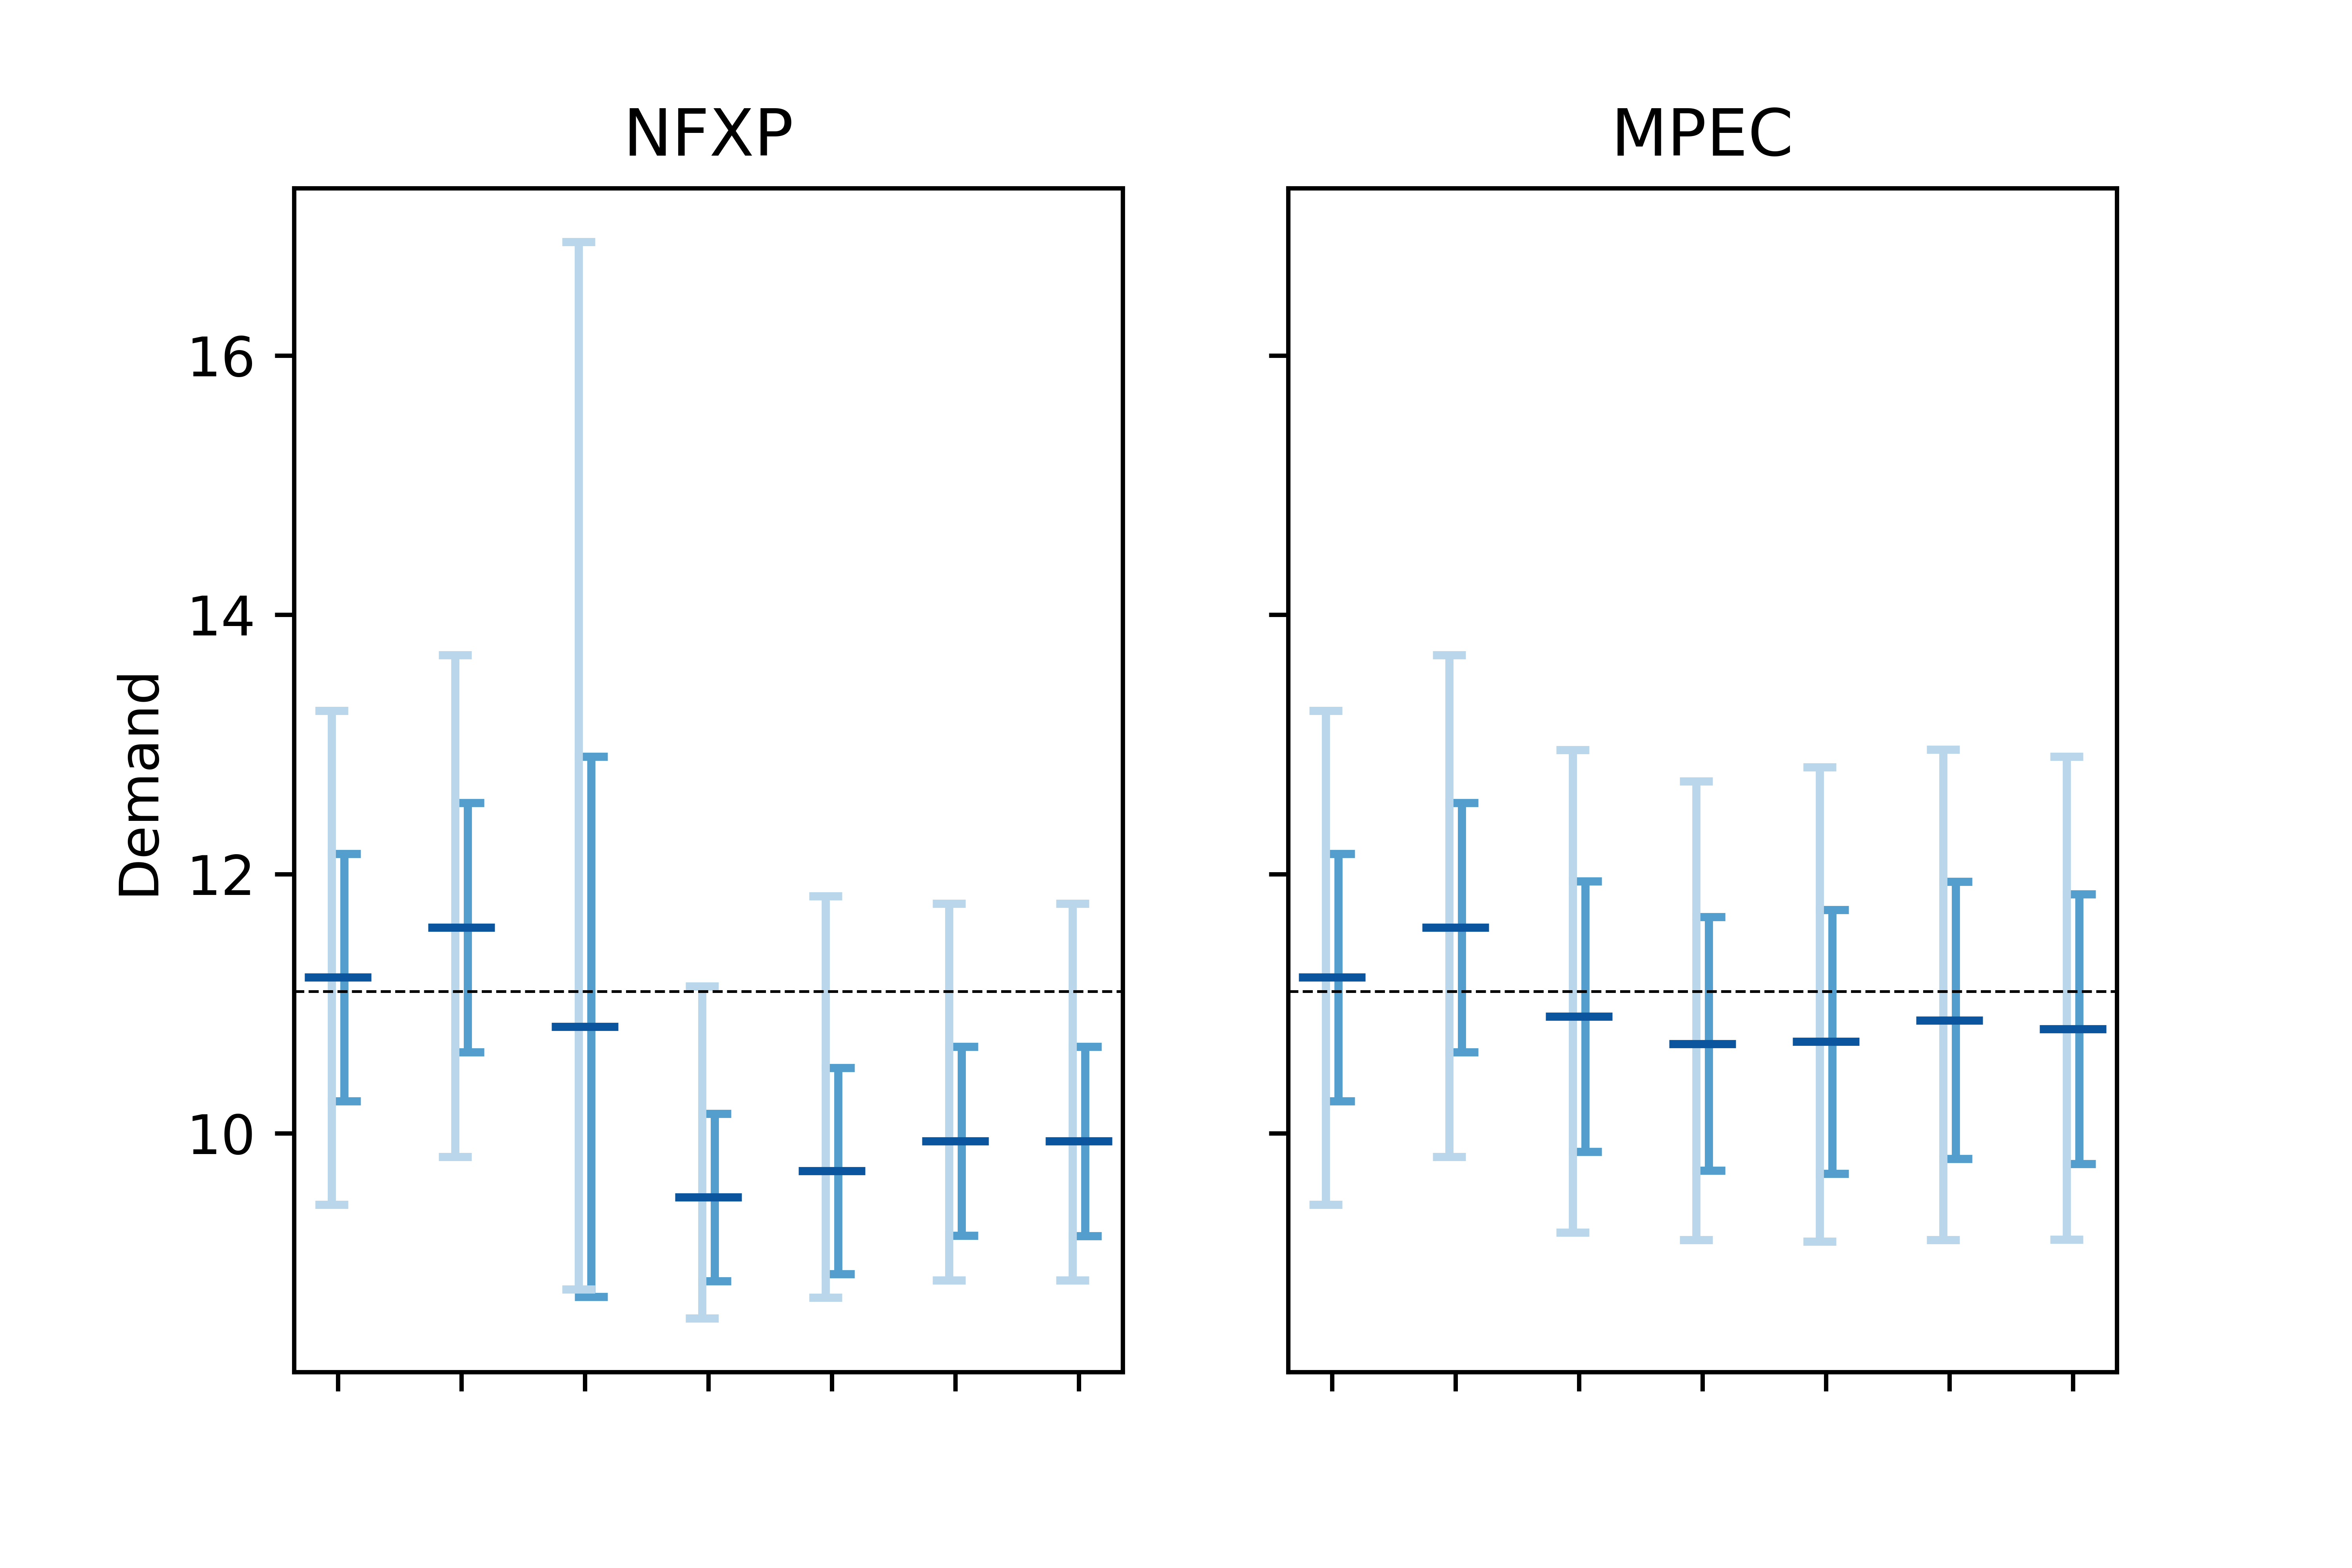
\includegraphics[scale=0.9]{../figures/figure_9.png}
	\label{figure9}
\end{figure}

\begin{figure}[H]
	\caption{Distribution of the QoI}
	\vspace*{-4mm}
	\centering
	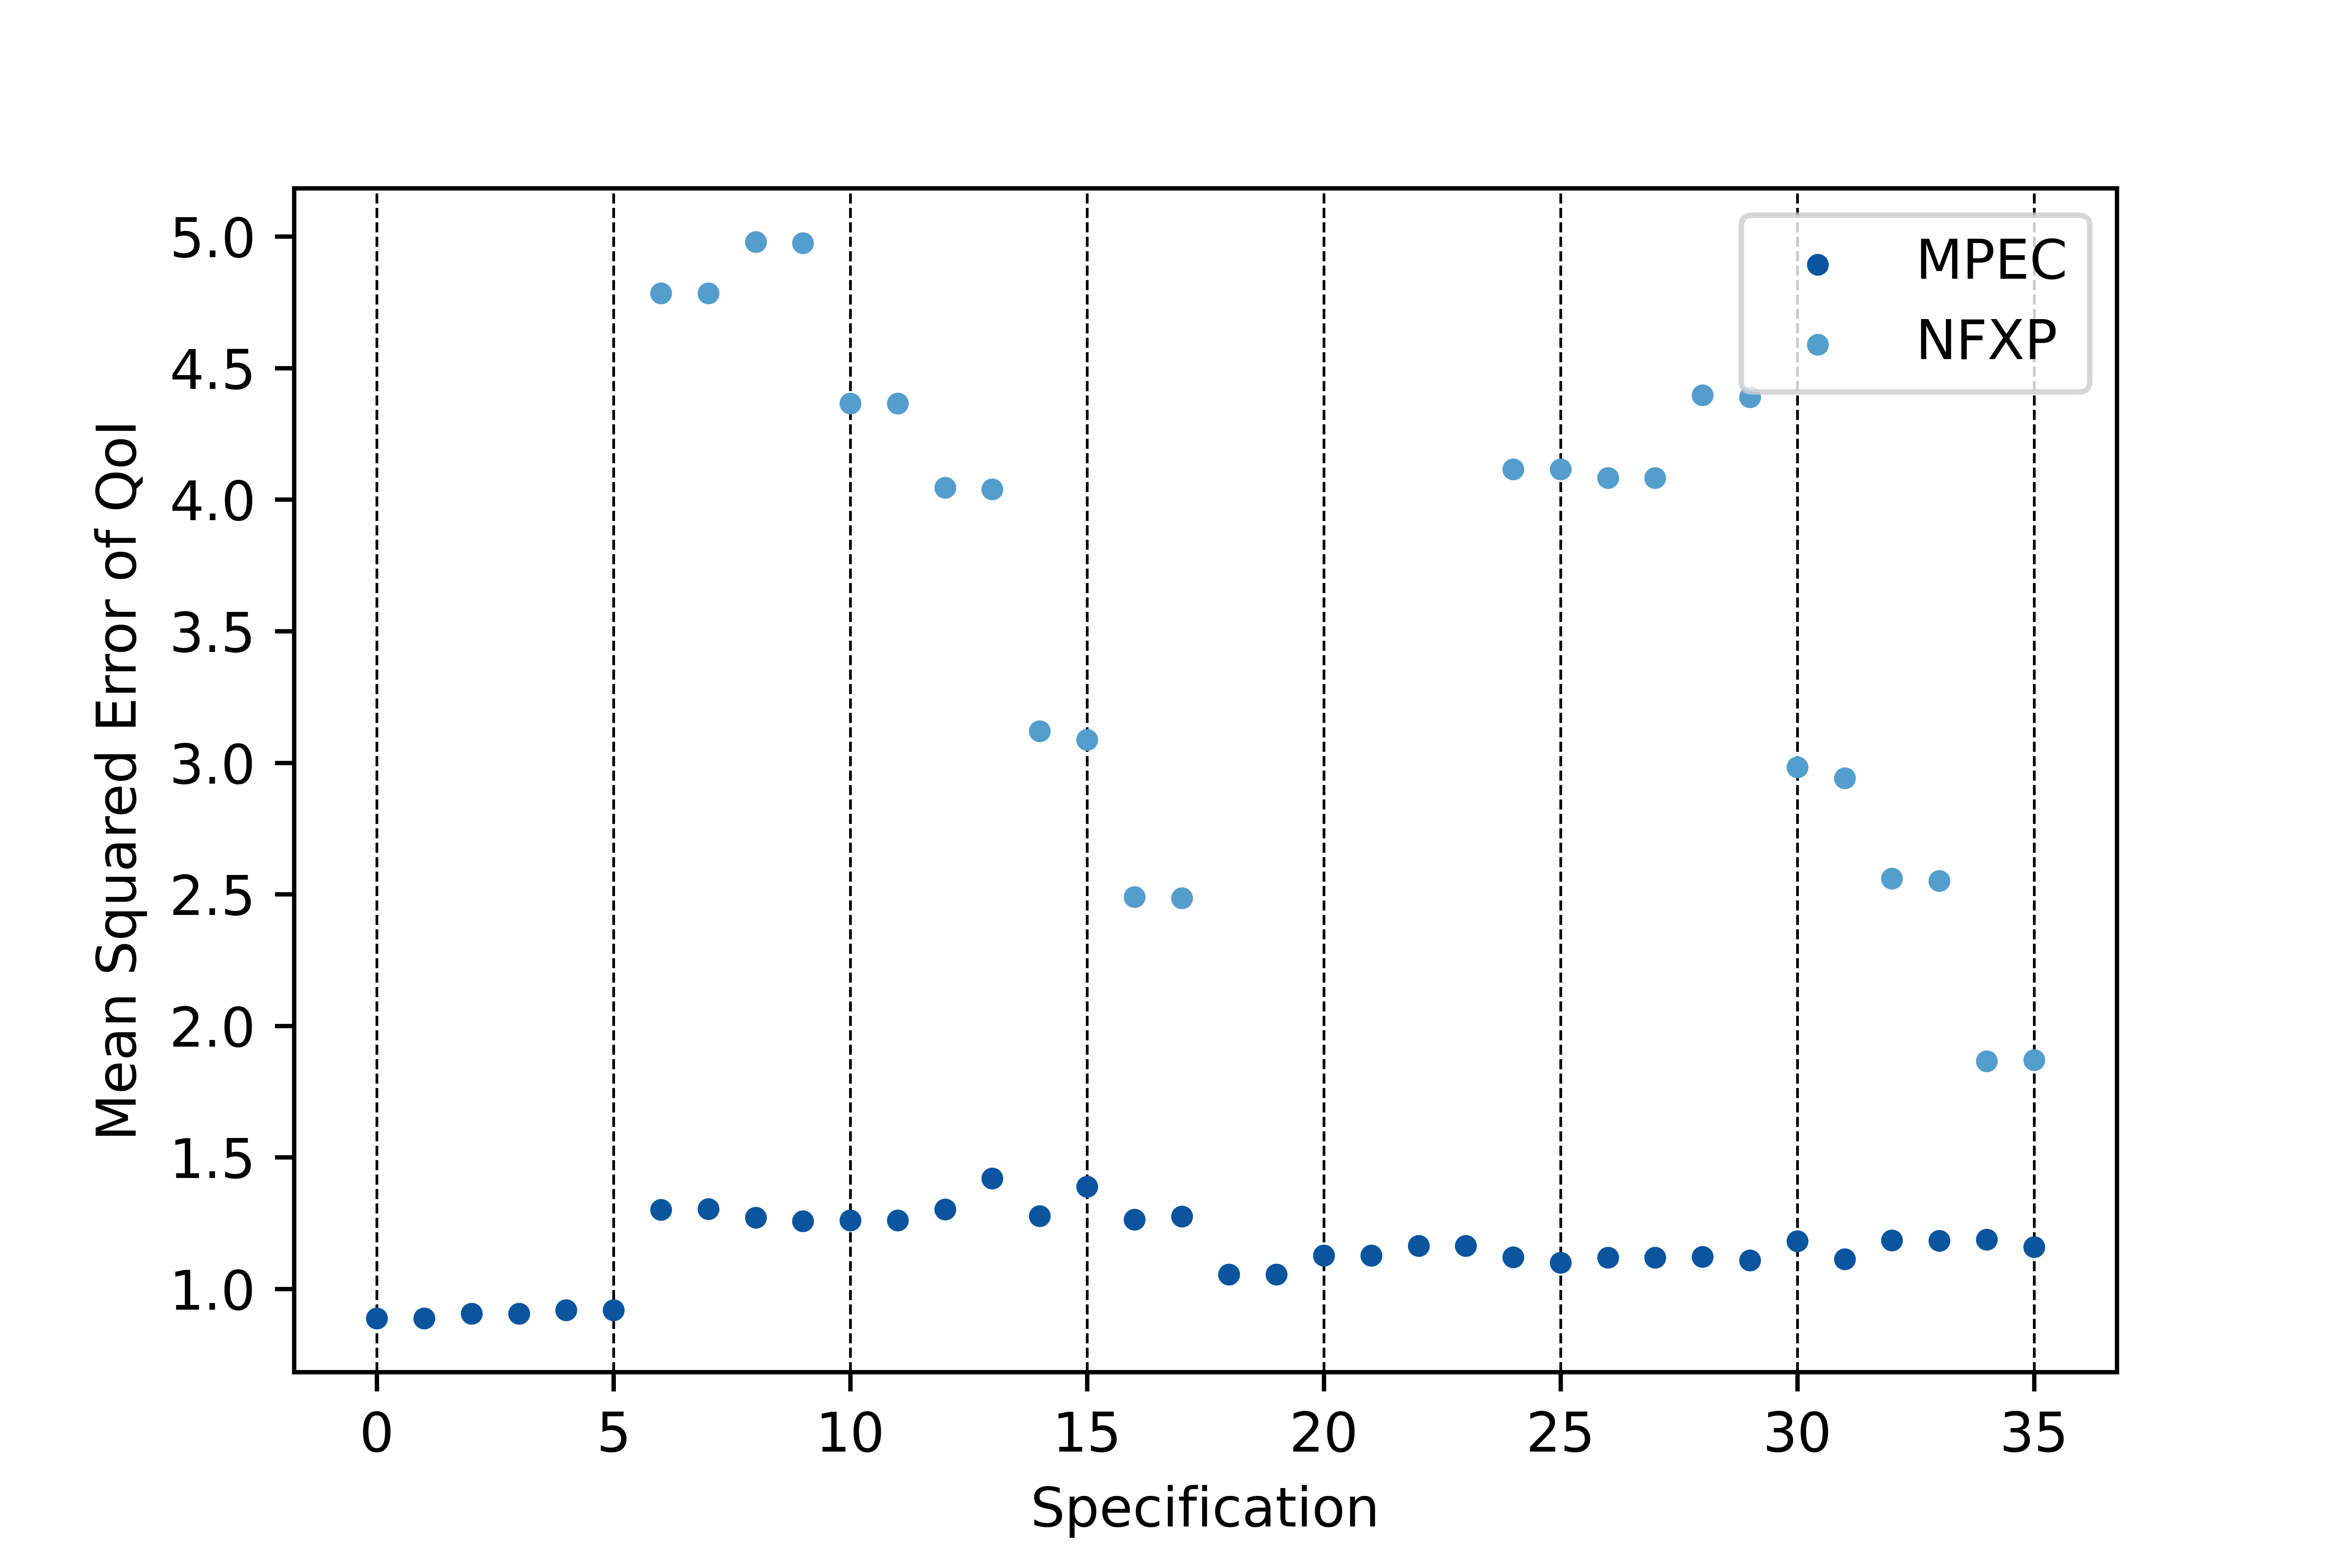
\includegraphics[scale=0.9]{../figures/figure_10.png}
	\label{figure10}
\end{figure}

\begin{figure}[H]
	\caption{Distribution of the QoI}
	\vspace*{-4mm}
	\centering
	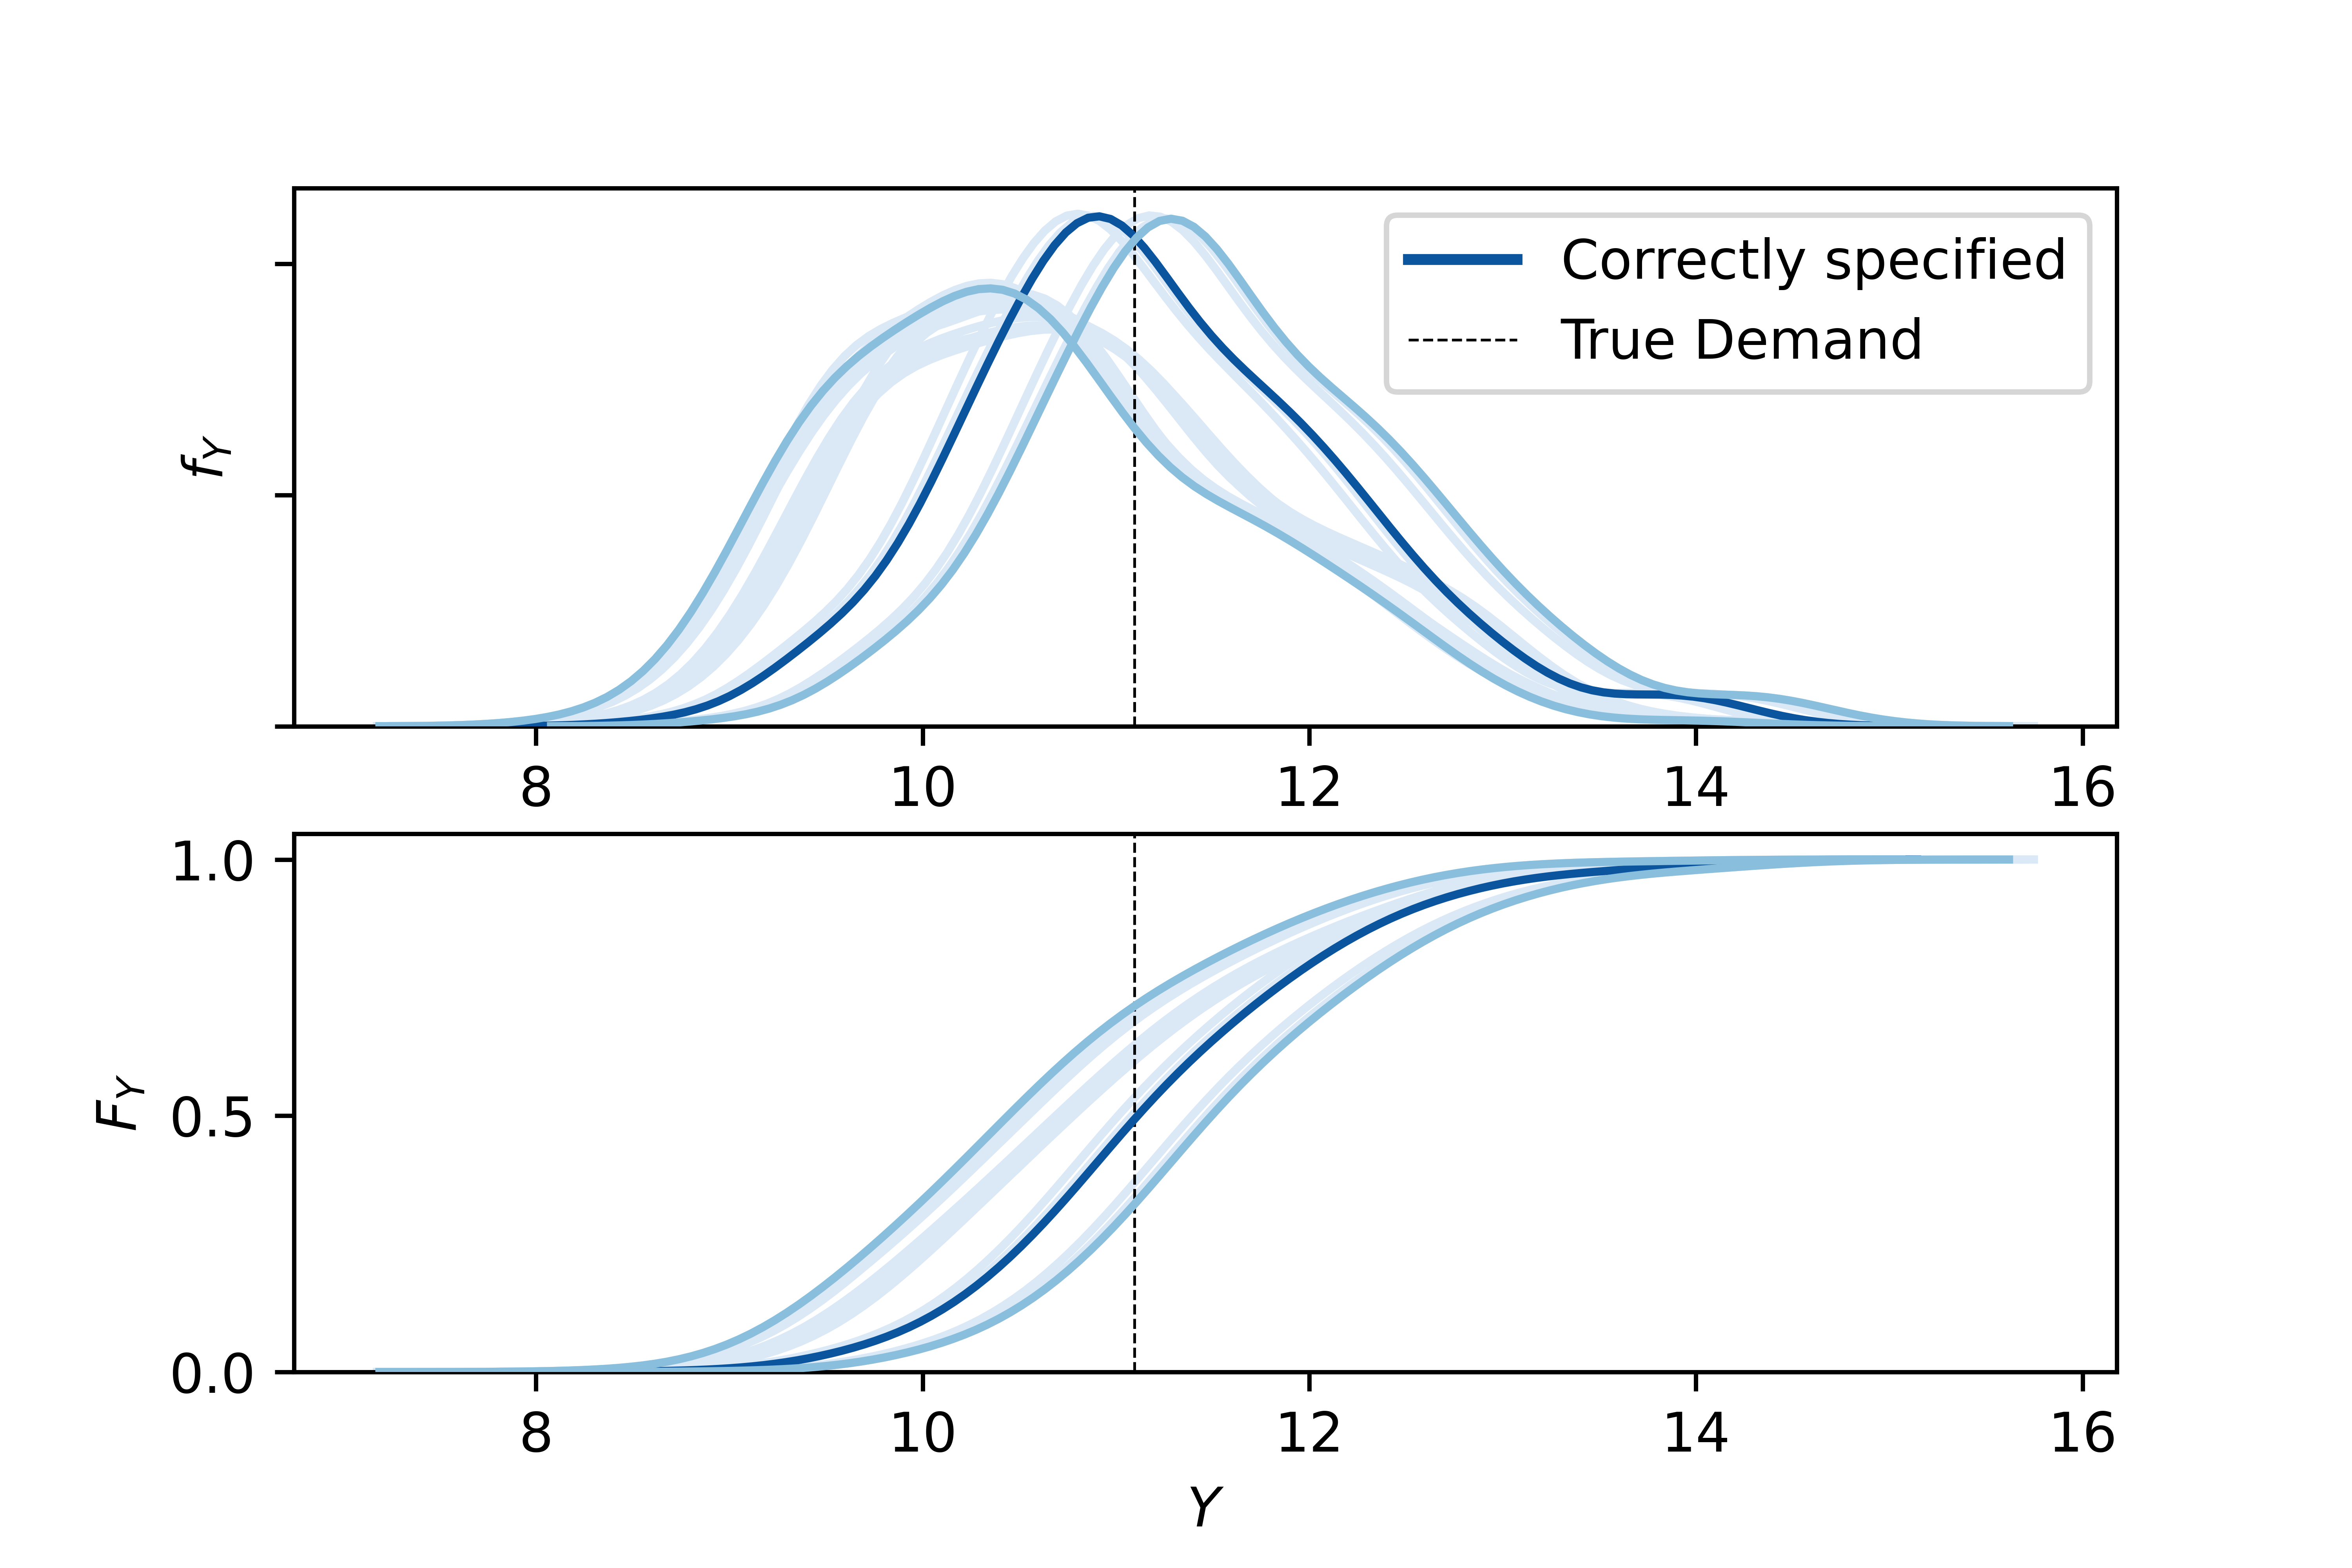
\includegraphics[scale=0.9]{../figures/figure_11.png}
	\label{figure11}
\end{figure}
